\chapter{System Analysis, Design \& Implementation}\label{chap3}

%##########################################
\vspace*{50 ex}

%##########################################
\paragraph*{Outline:} This chapter presents the following:
\begin{enumerate}
\setlength{\itemsep}{-0.3em}
\item Introduction
\item System Analysis
\item Design
\item Implementation
\end{enumerate}
\newpage

\section{Introduction}\label{chap3:intro}

In my proposed project \textbf{Social Media Android Application}, User can create account,post images and writes their description, sent messages,check status of his or his friends, see popular news and share those popular news.

\section{System Analysis}
System analysis consists following parts
\subsection{System Objective}
Communication over a network is one field where this tool finds wide ranging application. Chat application establishes a connection between 2 or more systems connected over an intranet or ad-hoc. This tool can be used for large scale communication and conferencing in an organization or campus of vast size, thus increasing the standard of co-operation. In addition it
converts the complex concept of sockets to a user friendly environment. This software can have
further potentials, such as file transfer, video calling and voice chatting options that can be worked upon later.
\subsection{Relation to External Environment}
This tool helps in two major aspects -
\bigskip
\begin{itemize}
	\item  Resolving the names of all the system connected in a network and enlisting them.
	\item Used for communication between multiple systems enlisted in the resolved list.

\end{itemize}

\subsection{ Design Considerations}
\textbf{Approach :}\\

\hfil
\hfil
The tool has been designed using XML \& Android in-build interface.\\

\noindent
\bigskip
\textbf{Methodology :}\\
	The user interacts with the tool using a GUI
\begin{itemize}
	\item The GUI operates in two forms, the List form \& the chat form.
	\item The List form contains the names of all the systems connected to a network.
	\item The chat form makes the actual communication possible in the form of text and images
\end{itemize}

\subsection{ System Architecture}
The chat application works in two forms..
\paragraph{List Form :}
In this form, all the names of the systems connected to a network are enlisted. These
names can later be used for communication with the help of touch on display, or in simple
language: texts or images.

\paragraph{Chat form :}
This form is called only when an element is selected from the List form. In this form, a
connection is created between the host system and the selected system with the help of a
socket. 
\paragraph{Flow Chart :}

\noindent
\begin{figure}[!ht]
	\centering
	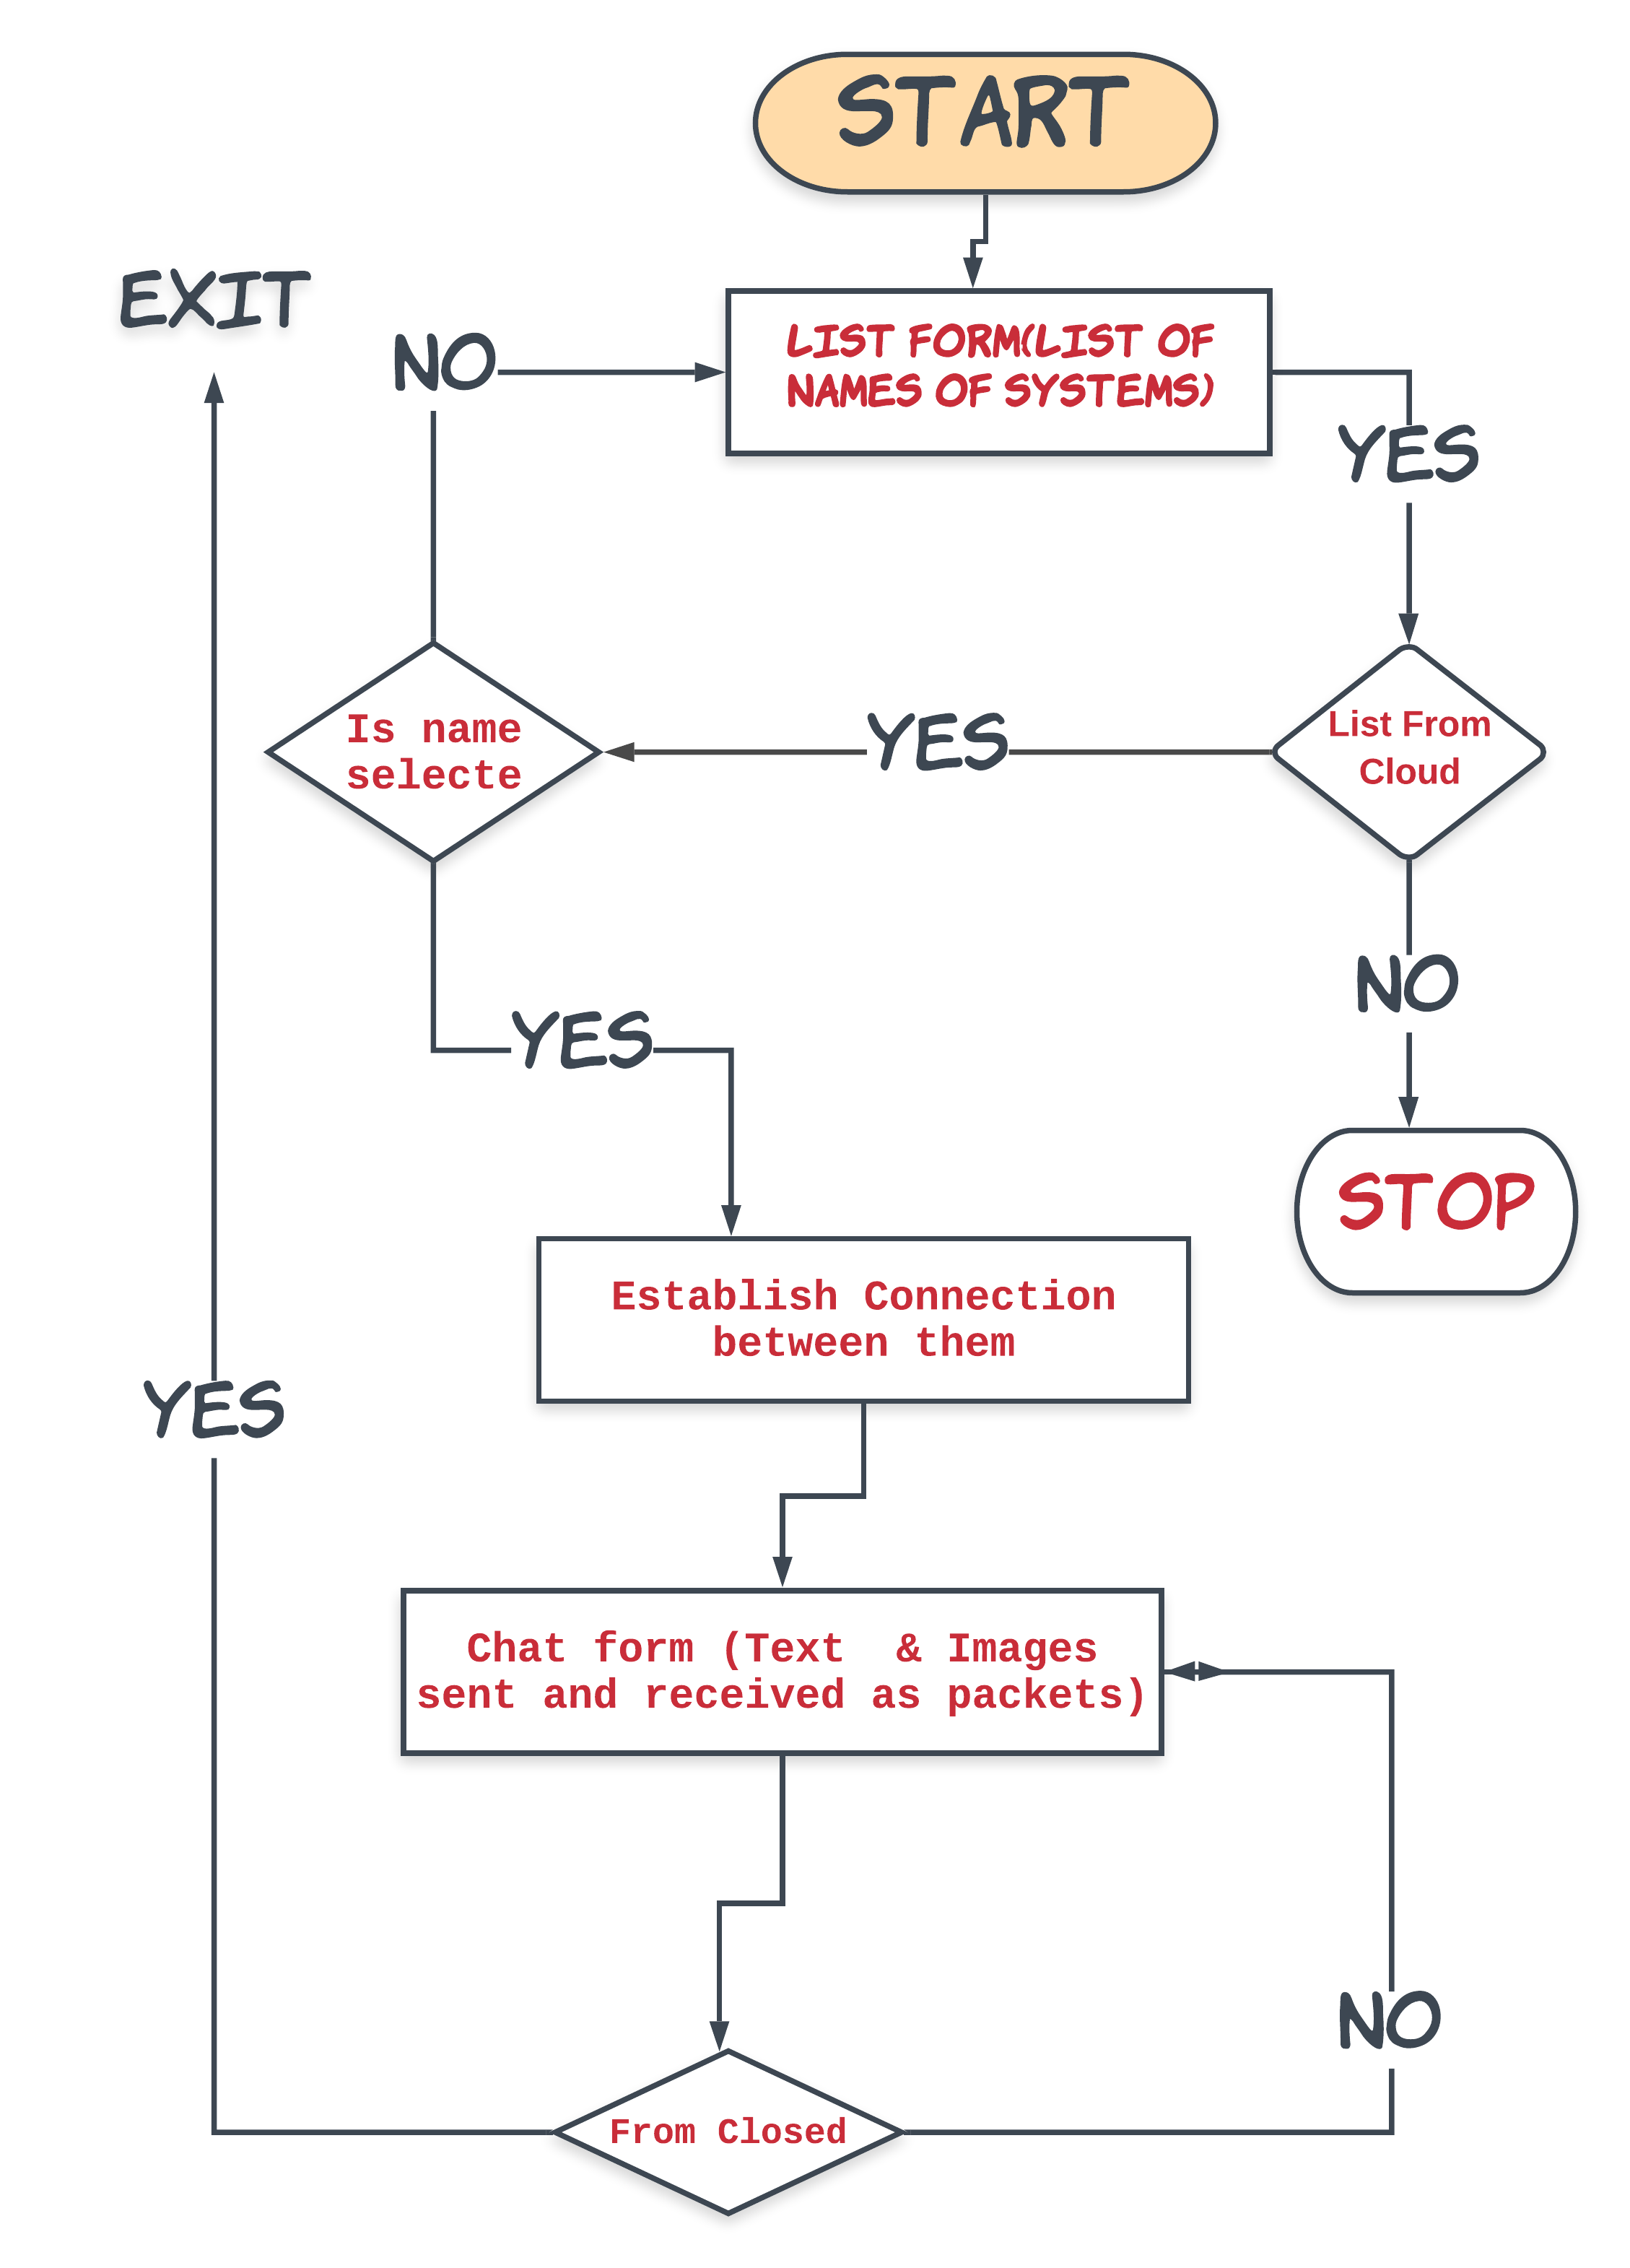
\includegraphics[scale=0.4]{flow-chart.png}
	\caption{\label{img1} Flow Chart}
\end{figure}
\vspace{70ex}
\subsection{ Operational Concepts and Scenarios}
Operation of the application based on the inputs given by the user:
\paragraph{List Form :}
\begin{itemize}
	\item When initialized, returns a list containing the names of all the system connected in a network.
	\item Contains two sections Refresh and Connect
	\item When Refresh section is auto refreshes the list of names.
	\item When the Connect section is worked properly or a name is clicked, the chat form is
	initialized with a connection between the host and the client machine.
	\item Note: If no name is selected, and connect section is clicked an error box is displayed.
\end{itemize}
\paragraph{Chat form :}
\begin{itemize}
	\item Contains a rich text-view which cannot be edited but only displays the messages from one user to another, including the self sent message, as in any chat application.
	\item Contains a text-view for messages to be written that is sent across the network.
	\item Contains messages and images Send buttons.
	\item When the sent button is clicked, in the background, the text in the text-view is encoded
	and sent as a packet over the network to the client machine. Here this message is
	decoded and is shown in the rich text-view.
	\item To make it more realistic, the self sent message is shown in the rich text-view as well. Both
	the messages is differentiated with the help of the identifier name at the beginning of each
	message in the rich text-view
\end{itemize}

\paragraph{Exit :}
The user exits the software in two scenarios:
\begin{itemize}
	\item Exits the chat form, the list form remains intact.
	\item Exits the list form, this is when the application is closed or user has been logout.
\end{itemize}
\section{Design}
My design phase includes :
\begin{enumerate}
	\setlength{\itemsep}{-0.3em}
	\item Flow Chart
	\item Data Flow Diagram
	\item Unified Modeling Language(UML)
	\item Database Design
	\item Implementation
\end{enumerate}
\subsection{Flow Chart}
\noindent
\begin{figure}[!ht]
	\centering
	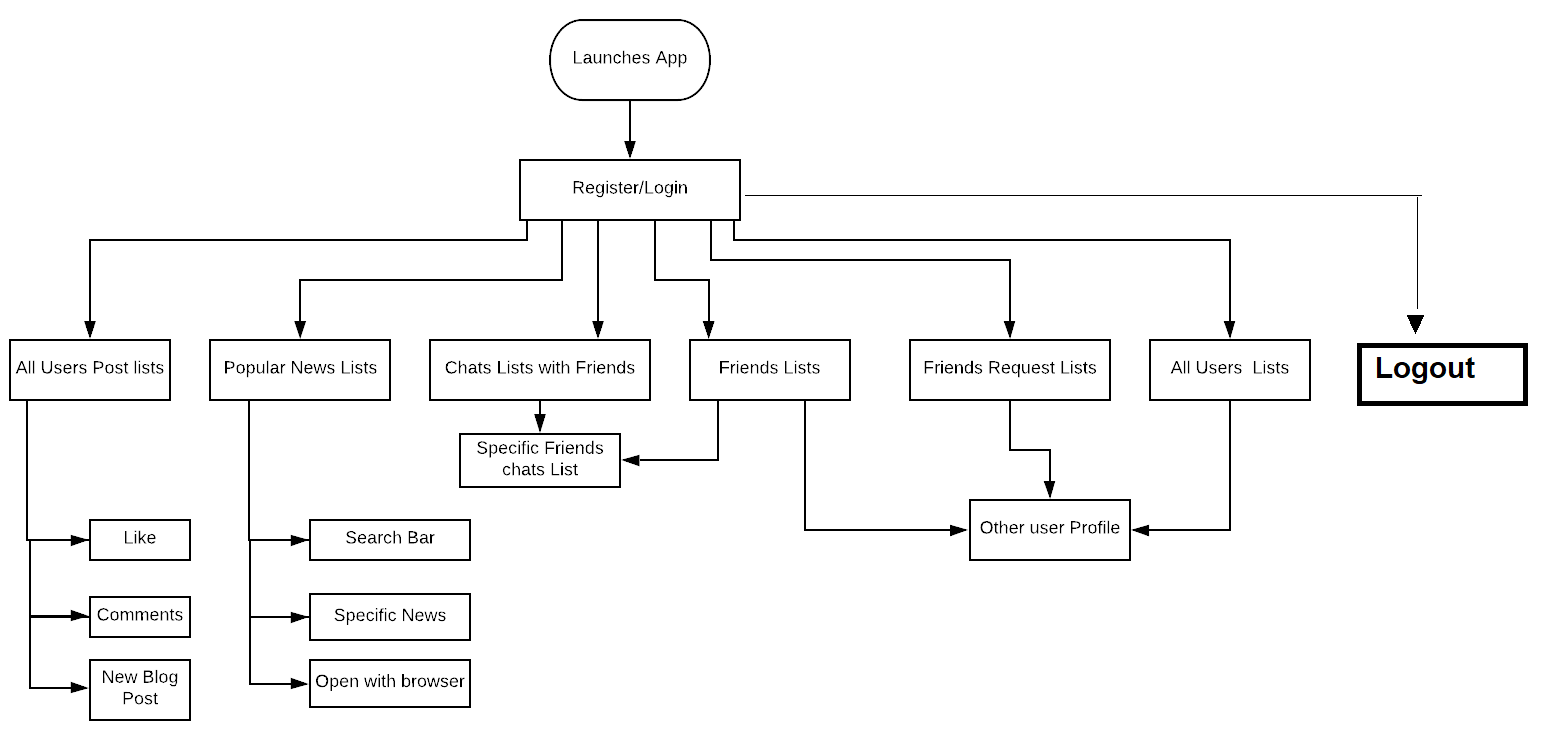
\includegraphics[scale=0.3]{flow-diagram.png}
	\caption{\label{img2} Flow Diagram}
\end{figure}

\noindent
The above diagram is the Flow diagram of this thesis. Here are the steps explained :-
\begin{enumerate}
	\setlength{\itemsep}{-0.3em}
	\item In the Above Diagram First of the user will enter its details then it will check
	for whether the provided details are correct or not if the user details are found
	correct then user will enter his or her home page activity and do the his or
	her required operations.\\
	\item As I have mentioned some of the features here which are of the user as he
	or she can search news, send friend request, accept friend request, chat with his friends, see his friends profile, all users status, find user form all users list, see blog post, like on post, comments on posts or add new blog posts.

\end{enumerate}

\subsection{Data Flow Diagram}

\subsubsection{User Case Table :}
\noindent
The below diagram is the User Case Table of this thesis. Here are the steps explained :-
\begin{enumerate}
	\setlength{\itemsep}{-0.3em}
	\item In the below diagram level 1 explains the feature of my proposed application.\\
	\item In the below diagram level 2 explains what does each sections of level 1.\\
	\item In the below diagram level 3 explains who will manage each sections.\\
	\item In the below diagram Admin means Database administrator
	
\end{enumerate}
\noindent
\begin{figure}[!ht]
		\centering
		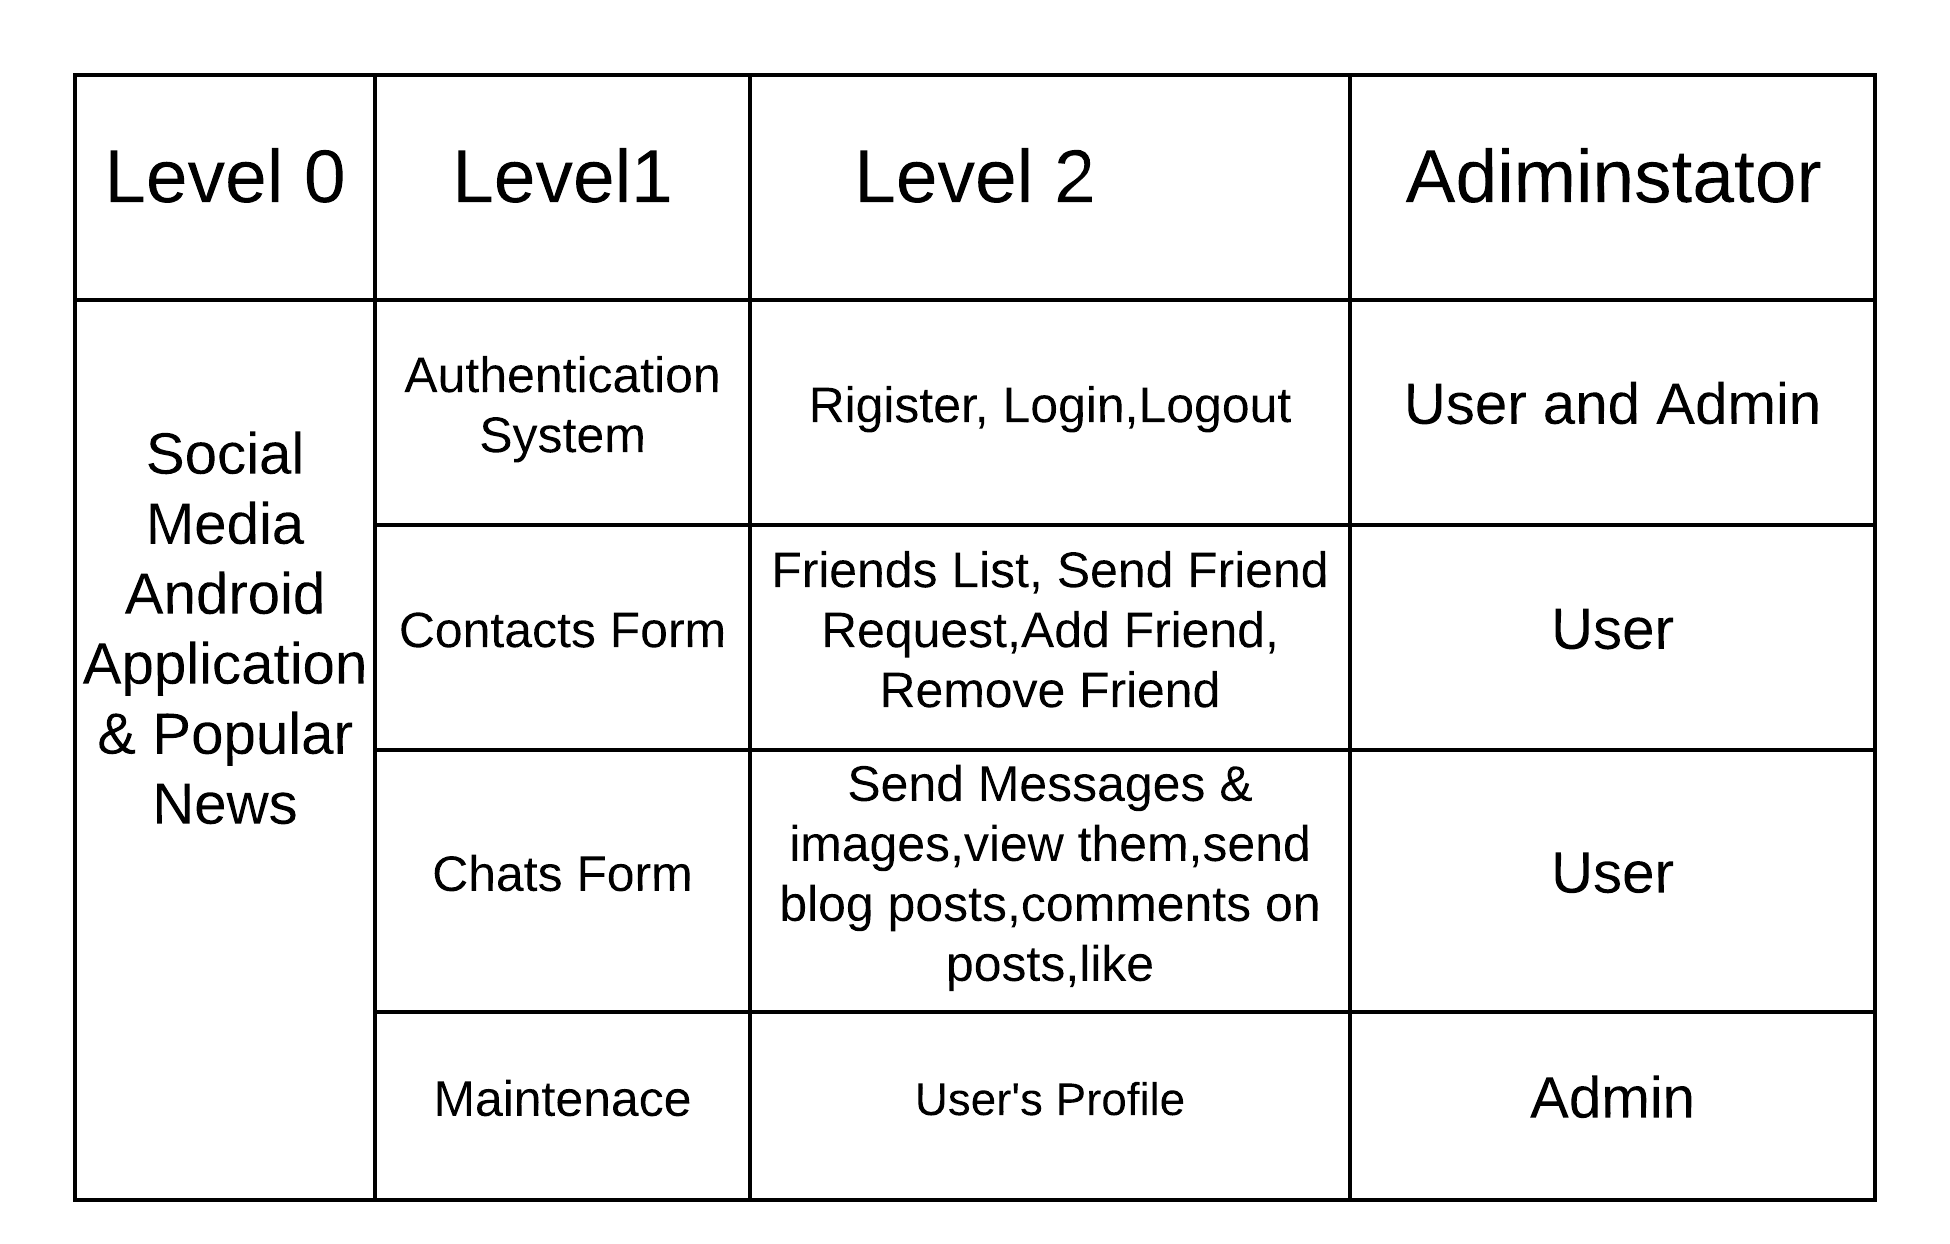
\includegraphics[scale=0.8]{user-table.png}
		\caption{\label{img3} User Case Table}
\end{figure}


\subsubsection{Authentication System :}
The below diagram is the authentication diagram of this thesis. Here are the steps explained :-
\begin{enumerate}
	\setlength{\itemsep}{-0.3em}
	\item In my proposed application user can register with the help of unique valid email-id, Name and their secure password.\\
	\item In this user can login with the help of unique email and their password.\\
	\item In this user can also logout.
	
\end{enumerate}
\noindent
\begin{figure}[!ht]
	\centering
	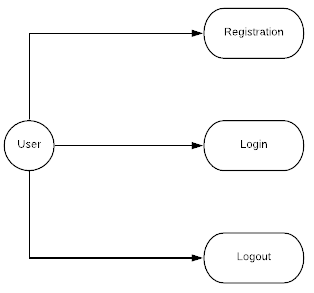
\includegraphics[scale=0.8]{auth.png}
	\caption{\label{img4}  Use Case Diagram of Authentication System}
\end{figure}
\noindent

\subsubsection{Contacts Form :}
\noindent
\begin{figure}[!ht]
	\centering
	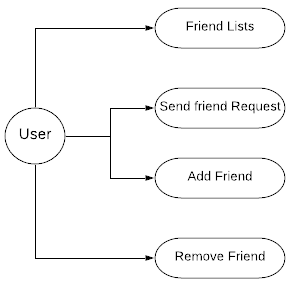
\includegraphics[scale=0.9]{friends.png}
	\caption{\label{img5}  Use Case Diagram of Contacts Form}
\end{figure}
\vspace{50ex}
\subsubsection{Chat Form :}
\noindent
\begin{figure}[!ht]
	\centering
	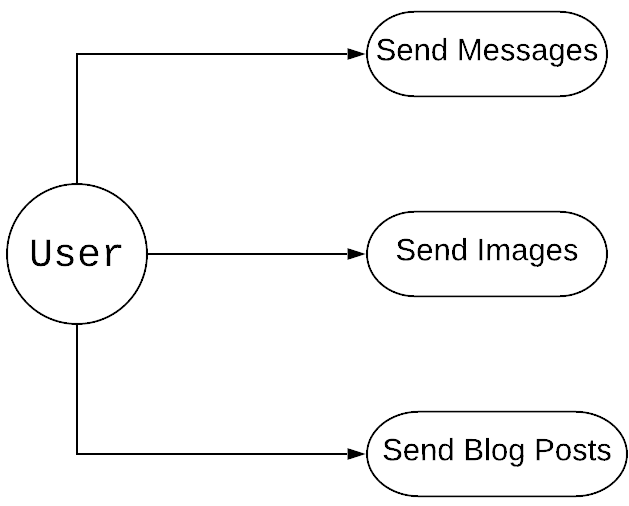
\includegraphics[scale=0.5]{chat-diagram.png}
	\caption{\label{img6}  Use Case Diagram of Chat Form}
\end{figure}



\subsubsection{Maintenance :}
\noindent
\begin{figure}[!ht]
	\centering
	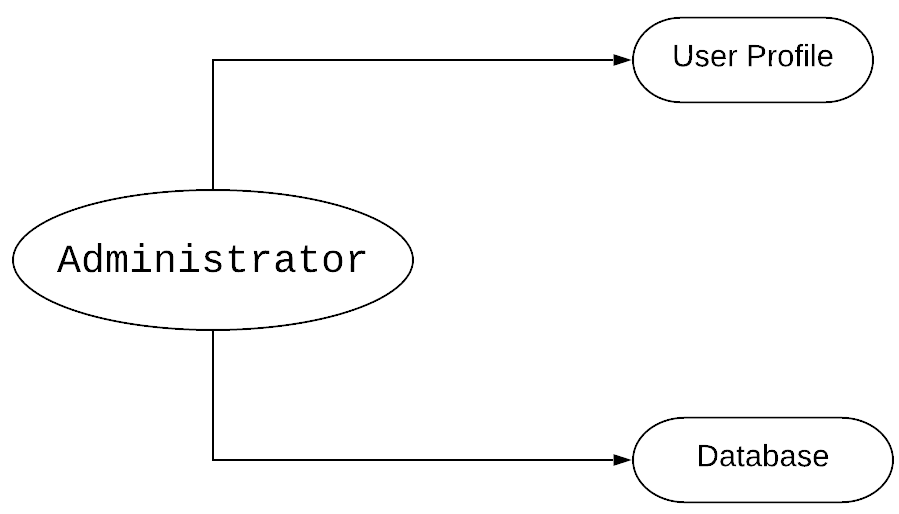
\includegraphics[scale=0.4]{maintenance.png}
	\caption{\label{img7}  Use Case Diagram of Maintenance}
\end{figure}
\vspace{50ex}
\subsection{UML Class Diagram}
Here is a Unified Modeling Language(UML) class diagram for this thesis which consists four classes user class, Account class, Blog\_Post class and Individual\_chat class and shows  composition of user class to their other classes

\begin{figure}[!ht]
	\centering
	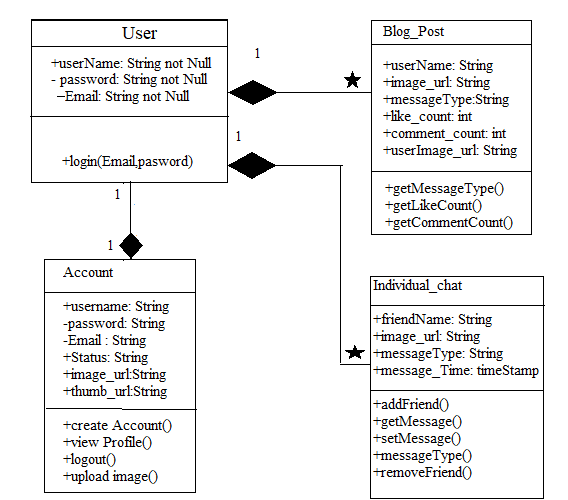
\includegraphics[scale=1]{project-uml.png}
	\caption{\label{img8}  UML Class diagram}
\end{figure}
\vspace{10ex}
\subsection{Database Design}
Here is the screenshot of my existing database...
\bigskip
\noindent

\begin{figure}[!ht]
	\centering
	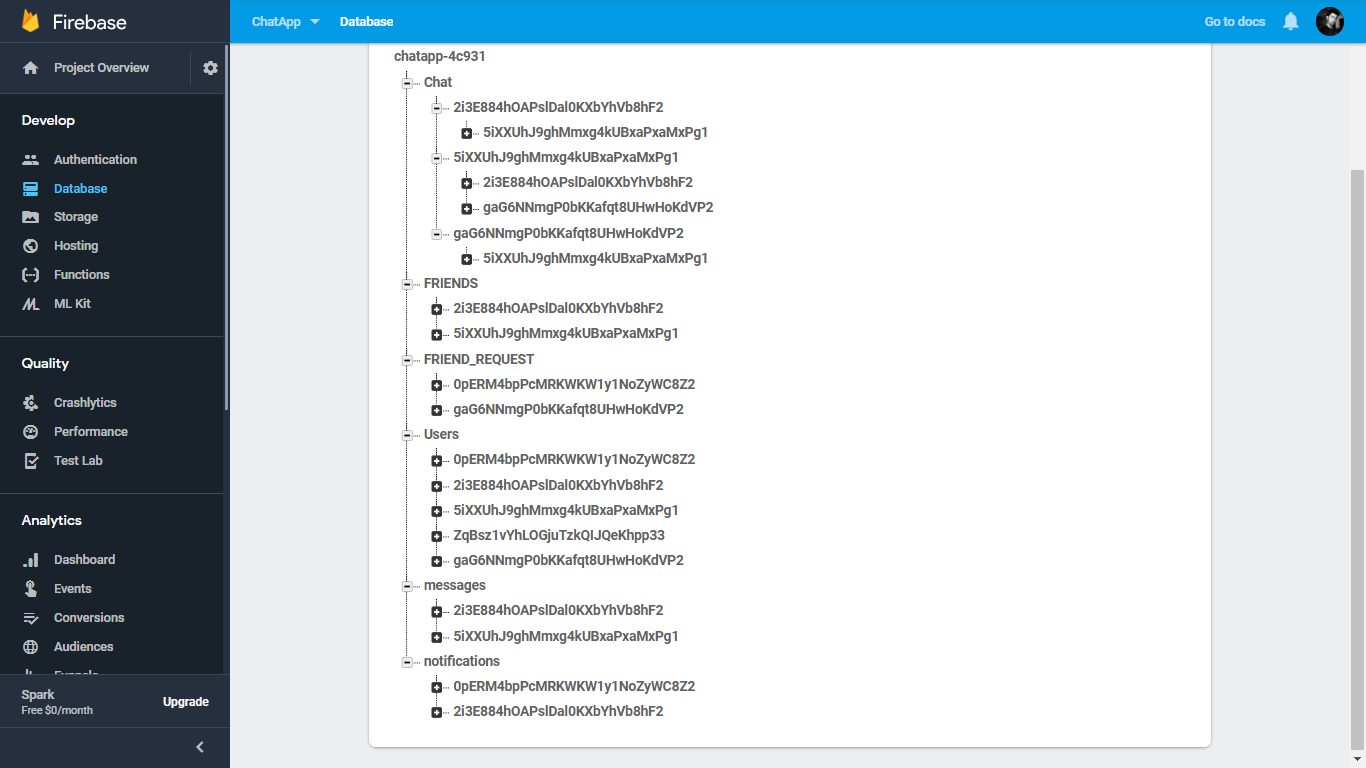
\includegraphics[scale=0.3]{databaseone.png}
	\caption{\label{img8}  Firebase users database text messages list}
\end{figure}
\vspace{10ex}
The above diagram is the real time database storage diagram which contains following informations...\\
\begin{enumerate}
	\setlength{\itemsep}{-0.3em}
	\item Users : Users Details like device token, users name, profile image URL, thumb-image URL, users status and his online status .\\
	\item FRIENDS : It contains users friends list\\
	\item {FRIENDS\_REQUEST : It contains users friend request type sent or received.\\}
	\item message : It contains users messages list with his friends.\\
	\item  notifications : When user send friend request it saves informations about friend request.\\
	\item Chat : It contains online or offline status of users. 
	
\end{enumerate}

\begin{figure}[!ht]
	\centering
	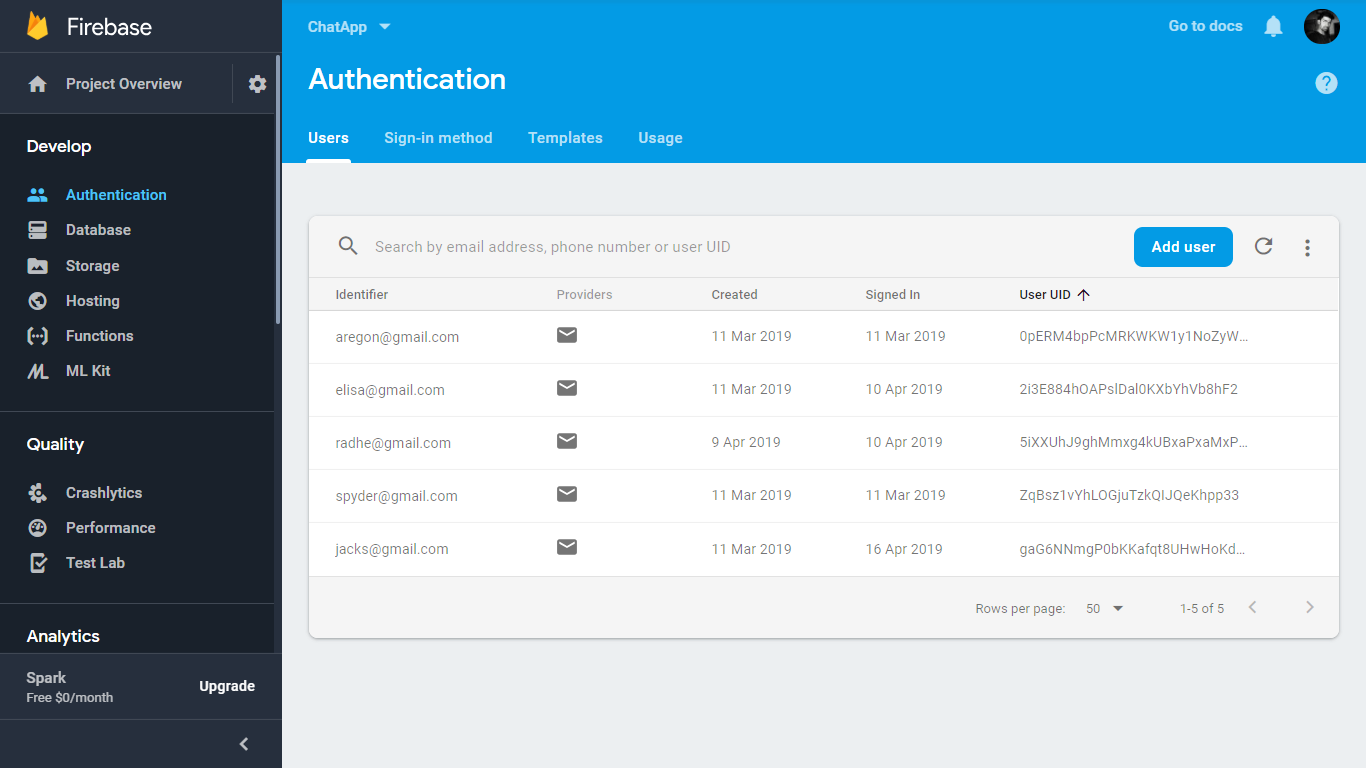
\includegraphics[scale=0.3]{databasetwo.png}
	\caption{\label{img9}  Firebase users authentication list}
\end{figure}
\noindent
The above diagram is authentication diagram which contains following informations
\begin{enumerate}
	\setlength{\itemsep}{-0.3em}
	\item Users valid email address.\\
	\item Users password which should be greater than 5 characters.\\
\end{enumerate}

\begin{figure}[!ht]
	\centering
	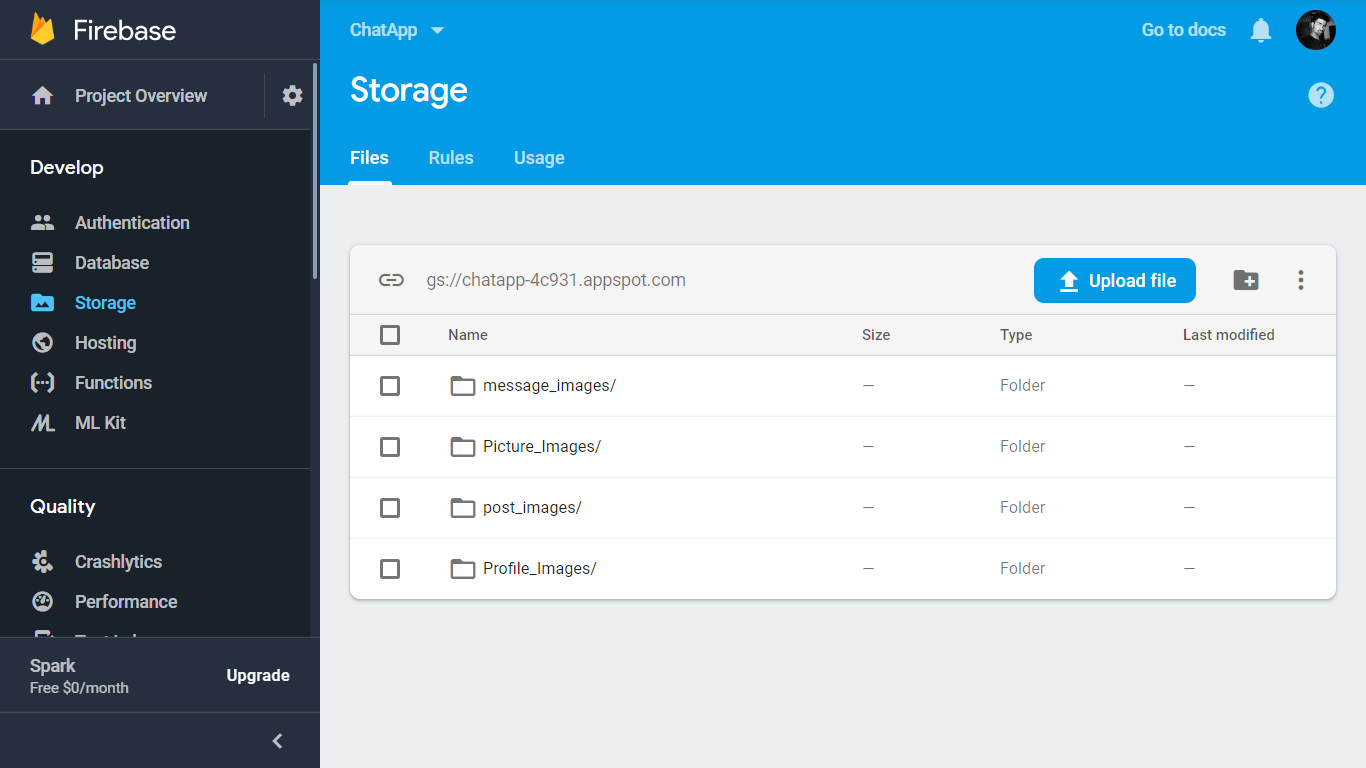
\includegraphics[scale=0.3]{databasethree.png}
	\caption{\label{img10}  Firebase storage folders list}
\end{figure}
\noindent
The below diagram is storage diagram which contains following informations
\begin{enumerate}
	\setlength{\itemsep}{-0.3em}
	\item message\_Images folder contains all chats related images .\\
	\item Profile\_Images contains thumb-images of all users.\\
	\item Picture\_images contains images of all users.\\
	\item post\_images contains blog post images. 
\end{enumerate}

\section{Implementation}
\subsection{Functional Requirements}

\begin{enumerate}
	\setlength{\itemsep}{-0.3em}
	\item User Registration : \\User must be able to register for the application through a valid Email Address. and password. On installing the application, user must be prompted to register with email, password and their name. If user skips this step, user will not be able to use this App. The users email will be the unique identifier of his/her account on this application.\\
	\item Send Message : \\User should be able to send instant message to any his/her friends and user will get notify when his friends will online by one green color image.\\
	\item Broadcast Message : \\ User should be able to post images and their description. User should be able
	to broadcast post to all users.\\
	\item Message Status :\\ User must be able to know on when the message has come and how much old it is.
\end{enumerate}

\subsection{Non Functional Requirements}

\begin{enumerate}
	\setlength{\itemsep}{-0.3em}
	\item Privacy :\\ Messages shared between users should be encrypted to maintain privacy\\
	\item Robustness : \\ In case users App crashes, a backup of their chat history must be
	stored on remote database servers to enable recoverability.
\\
	\item Performance : \\ Application must be lightweight and must send messages instantly.\\
\end{enumerate}

%\section{Summary}
%In this chapter...